\chapter{Contact Forces, Solid Friction, and Mechanical Constraints}
\label{ch:friction_constraints}

\begin{chapterintro}
\textbf{Chapter Objectives:} Contact forces transmit the interactions that prevent matter from interpenetrating. In this chapter, you will master the Amontons-Coulomb laws of dry friction; construct the friction cone; derive the exponential Capstan formula for ropes wound around cylinders; analyze banked turns; and solve multi-tier stacked body problems with static and kinetic thresholds.
\end{chapterintro}

\section{The Nature of Contact Forces}

When two physical bodies touch, the microscopic electrostatic repulsion between electron clouds in their outer atomic layers prevents interpenetration. At the macroscopic scale, this distributed contact stress is resolved into two orthogonal components:
\[
\boxed{\vec{R} = \vec{N} + \vec{f},}
\]
where:
\begin{itemize}[leftmargin=1.4em,itemsep=3pt]
  \item $\vec{N}$ is the \textbf{Normal Force}, perpendicular to the contact tangent plane, preventing interpenetration ($N \ge 0$).
  \item $\vec{f}$ is the \textbf{Frictional Force}, parallel to the contact tangent plane, opposing relative sliding.
\end{itemize}

\begin{figure}[htbp]
\centering
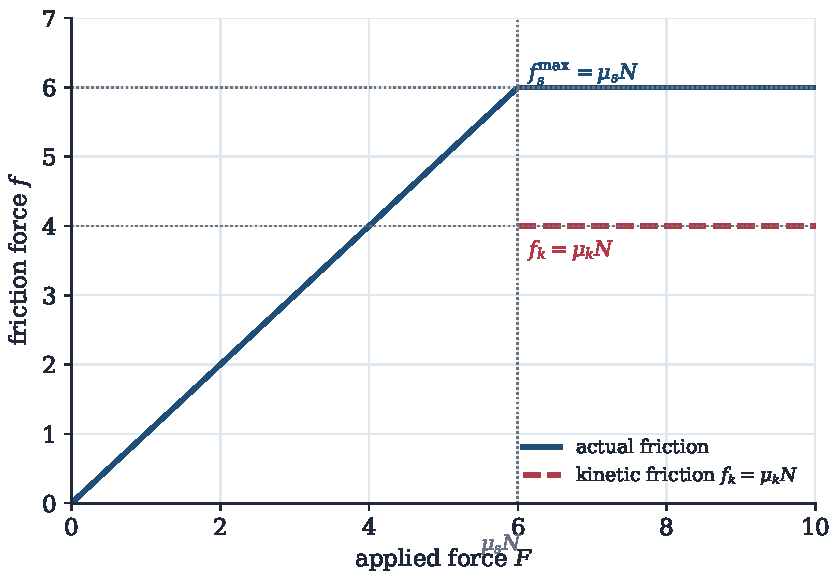
\includegraphics[width=0.74\textwidth]{figures/13_friction.pdf}
\caption{The classic friction response curve. As tangential force $F$ increases, static friction matches it identically until the peak $\mu_s N$. Once sliding begins, kinetic friction drops to the constant level $\mu_k N$.}
\label{fig:friction_curve}
\end{figure}

\section{The Amontons-Coulomb Laws of Dry Friction}

Formulated experimentally by Guillaume Amontons (1699) and refined by Charles-Augustin de Coulomb (1781):
\begin{lawbox}{Coulomb's Laws of Solid Friction}
\begin{enumerate}[leftmargin=1.5em,itemsep=3pt]
  \item \textbf{Static Friction ($v_{\text{rel}} = 0$)}: Prevents the initiation of sliding. It acts as an adjustable constraint force matching the applied tangential load up to a sharp threshold:
        \[
        \boxed{f_s \le \mu_s\,N,}
        \]
        where $\mu_s$ is the dimensionless \textbf{coefficient of static friction}.
  \item \textbf{Kinetic Friction ($v_{\text{rel}} \ne 0$)}: Resists established sliding motion, oriented strictly opposite to the relative velocity:
        \[
        \boxed{\vec{f}_k = -\mu_k\,N\,\frac{\vec{v}_{\text{rel}}}{\norm{\vec{v}_{\text{rel}}}},}
        \]
        where $\mu_k$ is the \textbf{coefficient of kinetic friction}. In virtually all physical material pairings, $\mu_k < \mu_s$.
  \item \textbf{Area Independence}: To a remarkable approximation, $f$ is independent of the apparent geometric contact area between the surfaces.
\end{enumerate}
\end{lawbox}

\begin{figure}[htbp]
\centering
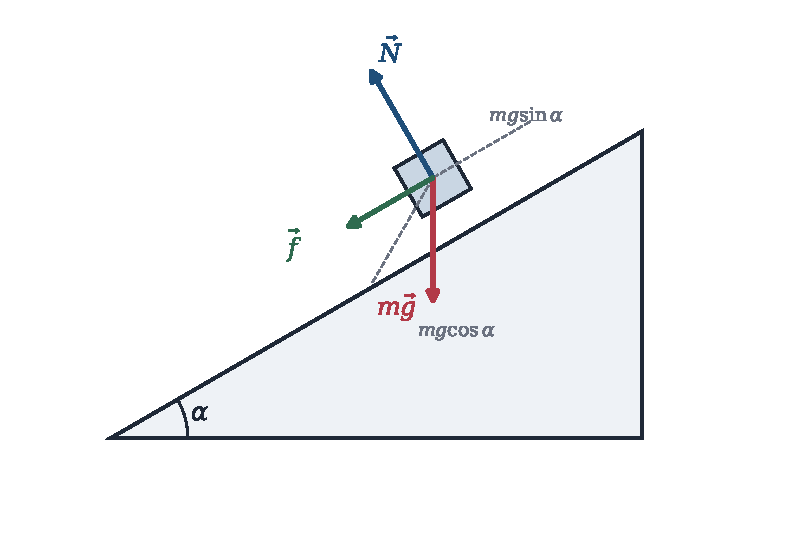
\includegraphics[width=0.74\textwidth]{figures/11_incline_fbd.pdf}
\caption{Free-Body Diagram of a block on a rough incline of angle $\alpha$. Normal force $N = mg\cos\alpha$ and friction $f$ oppose gravity's downhill pull $mg\sin\alpha$.}
\label{fig:incline_fbd}
\end{figure}

\begin{definitionbox}{The Friction Cone and Angle of Repose}
The total contact reaction vector $\vec{R} = \vec{N} + \vec{f}$ makes an angle $\phi$ with the normal:
\[
\tan\phi = \frac{f}{N}.
\]
At the threshold of impending motion ($f = \mu_s N$), the angle reaches its maximum value $\phi_s$:
\[
\boxed{\tan\phi_s = \mu_s.}
\]
The cone of half-angle $\phi_s$ around the normal is the \textbf{Friction Cone}. If the resultant applied external load falls inside this cone, sliding is physically impossible regardless of how large the force is!
The \textbf{angle of repose} $\alpha_c$ of an incline is precisely $\alpha_c = \phi_s = \arctan\mu_s$.
\end{definitionbox}

\section{Extensive Worked Examples}

\begin{workedexample}{Minimum Force to Pull a Crate on a Rough Floor}
A heavy crate of mass $m$ rests on a rough horizontal floor with static friction coefficient $\mu_s$. A rope pulls the crate with force $\vec{F}$ inclined at angle $\theta$ above the horizontal.
(a) Find the magnitude of force $F(\theta)$ required to initiate motion.
(b) Find the optimal pulling angle $\theta_{\text{opt}}$ that minimizes the required pulling force $F$, and calculate $F_{\min}$.

\paragraph{Solution.}

(a) Set up horizontal and vertical axes:
\begin{align*}
\text{Vertical balance:}\quad & N + F\sin\theta - mg = 0 \implies N = mg - F\sin\theta, \\
\text{Horizontal balance:}\quad & F\cos\theta - f_s = 0 \implies f_s = F\cos\theta.
\end{align*}
Sliding begins when static friction reaches its maximum threshold $f_s = \mu_s N$:
\[
F\cos\theta = \mu_s(mg - F\sin\theta) = \mu_s mg - \mu_s F\sin\theta.
\]
Rearranging terms:
\[
F(\cos\theta + \mu_s\sin\theta) = \mu_s mg \implies \boxed{F(\theta) = \frac{\mu_s mg}{\cos\theta + \mu_s\sin\theta}.}
\]

(b) To minimize $F(\theta)$, we maximize the denominator $D(\theta) = \cos\theta + \mu_s\sin\theta$.
Differentiating with respect to $\theta$:
\[
D'(\theta) = -\sin\theta + \mu_s\cos\theta = 0 \implies \boxed{\tan\theta_{\text{opt}} = \mu_s.}
\]
The optimal pulling angle is precisely equal to the \textbf{angle of friction} $\phi_s$!
At this optimal angle:
\[
\cos\theta_{\text{opt}} = \frac{1}{\sqrt{1 + \mu_s^2}}, \qquad \sin\theta_{\text{opt}} = \frac{\mu_s}{\sqrt{1 + \mu_s^2}}.
\]
The maximum denominator value is:
\[
D(\theta_{\text{opt}}) = \frac{1}{\sqrt{1 + \mu_s^2}} + \frac{\mu_s^2}{\sqrt{1 + \mu_s^2}} = \frac{1 + \mu_s^2}{\sqrt{1 + \mu_s^2}} = \sqrt{1 + \mu_s^2}.
\]
Therefore, the absolute minimum force required is:
\[
\boxed{F_{\min} = \frac{\mu_s mg}{\sqrt{1 + \mu_s^2}} = mg\sin\phi_s.}
\]
Pulling slightly upward reduces the normal force $N$, which dramatically reduces friction, requiring much less effort than pulling horizontally ($F(0) = \mu_s mg$).
\end{workedexample}

\begin{workedexample}{The Capstan Equation (Belt Friction)}
A flexible rope is wrapped around a fixed rough horizontal cylinder of circular cross-section with coefficient of friction $\mu$. The rope subtends a total contact wrap angle $\theta$ (in radians).
A tension $T_1$ is applied to one end.
Prove the celebrated \textbf{Eytelwein--Capstan Formula} for the maximum holding tension $T_2$ at the other end before slipping:
\[
T_2 = T_1\,e^{\mu\theta}.
\]

\paragraph{Solution.}

Isolate an infinitesimal segment of the rope subtending an angle $\dd\theta$:
\begin{itemize}[leftmargin=1.4em,itemsep=2pt]
  \item Tension at angle $\theta$: $T$.
  \item Tension at angle $\theta + \dd\theta$: $T + \dd T$.
  \item Normal reaction from the cylinder: $\dd N$ directed radially outward.
  \item Maximum static friction force: $\dd f = \mu\,\dd N$ directed along the tangent opposing slipping.
\end{itemize}
Projecting forces along the radial and tangential directions:
\begin{align*}
\text{Radial:}\quad & \dd N - (T + \dd T)\sin\left(\frac{\dd\theta}{2}\right) - T\sin\left(\frac{\dd\theta}{2}\right) = 0.
\end{align*}
For infinitesimal angles, $\sin(\dd\theta/2) \approx \dd\theta/2$:
\[
\dd N = 2T\frac{\dd\theta}{2} + \dd T\frac{\dd\theta}{2} \approx T\,\dd\theta.
\]
(The second-order term $\dd T\dd\theta$ is discarded).

Projecting along the tangential direction:
\begin{align*}
\text{Tangential:}\quad & (T + \dd T)\cos\left(\frac{\dd\theta}{2}\right) - T\cos\left(\frac{\dd\theta}{2}\right) - \dd f = 0.
\end{align*}
With $\cos(\dd\theta/2) \approx 1$ and $\dd f = \mu\,\dd N$:
\[
\dd T = \dd f = \mu\,\dd N.
\]
Substitute $\dd N = T\,\dd\theta$:
\[
\dd T = \mu\,T\,\dd\theta \implies \frac{\dd T}{T} = \mu\,\dd\theta.
\]
Integrating across the entire wrap angle from $\theta = 0$ (tension $T_1$) to angle $\theta$ (tension $T_2$):
\[
\int_{T_1}^{T_2} \frac{\dd T}{T} = \mu\int_0^\theta \dd\theta' \implies \ln\left(\frac{T_2}{T_1}\right) = \mu\theta.
\]
Exponentiating both sides yields the famous \textbf{Capstan Equation}:
\[
\boxed{T_2 = T_1\,e^{\mu\theta}.}
\]
\textbf{Remarkable Physical Consequence:}
Because of the exponential dependence, friction grows extraordinarily fast with the number of turns $n$ ($\theta = 2\pi n$).
For a rope on an iron bollard with $\mu = 0.40$ wrapped $3$ full turns ($n = 3 \implies \theta = 6\pi \approx 18.85\ \mathrm{rad}$):
\[
\frac{T_2}{T_1} = e^{0.40\times 18.85} = e^{7.54} \approx \mathbf{1882.}
\]
A single sailor holding the line with a gentle force of $T_1 = 50\ \mathrm{N}$ (about $5\ \mathrm{kg}$ of pull) can hold a massive ship exerting $T_2 = 1882\times 50 \approx \mathbf{94\,100\ \mathrm{N}}$ (equivalent to nearly $10$ metric tons)!
\end{workedexample}

\begin{workedexample}{Maximum Cornering Speed on a Banked Highway}
A civil engineer designs a highway curve of radius $R = 200\ \mathrm{m}$ banked at an angle $\theta = 15.0^\circ$. The coefficient of static friction between car tires and the road surface is $\mu_s = 0.500$.
(a) Find the \textbf{rated speed} $v_0$ for which no friction is needed to negotiate the turn safely.
(b) Find the maximum speed $v_{\max}$ before the car slips up the bank.
(c) Find the minimum speed $v_{\min}$ below which the car slides down the bank.

\paragraph{Solution.}

(a) Rated speed ($f = 0$):
Gravity pulls down ($-mg$), and the normal force $\vec{N}$ provides both vertical support and horizontal centripetal acceleration:
\begin{align*}
N\cos\theta &= mg, \\
N\sin\theta &= m\frac{v_0^2}{R}.
\end{align*}
Dividing gives $\tan\theta = \frac{v_0^2}{gR}$:
\[
\boxed{v_0 = \sqrt{gR\tan\theta}.}
\]
Computing:
\[
v_0 = \sqrt{(9.81)(200)\tan 15.0^\circ} = \sqrt{1962\times 0.2679} = \sqrt{525.7} \approx \mathbf{22.9\ \mathrm{m\,s^{-1}}} \approx 82.5\ \mathrm{km\,h^{-1}}.
\]

(b) Maximum speed $v_{\max}$ (impending slip up the bank):
Friction points down the incline: $f_s = \mu_s N$.
Equations of motion:
\begin{align*}
\text{Vertical:}\quad & N\cos\theta - \mu_s N\sin\theta = mg \implies N(\cos\theta - \mu_s\sin\theta) = mg, \\
\text{Horizontal:}\quad & N\sin\theta + \mu_s N\cos\theta = m\frac{v_{\max}^2}{R} \implies N(\sin\theta + \mu_s\cos\theta) = m\frac{v_{\max}^2}{R}.
\end{align*}
Dividing the two equations:
\[
\frac{v_{\max}^2}{gR} = \frac{\sin\theta + \mu_s\cos\theta}{\cos\theta - \mu_s\sin\theta} = \frac{\tan\theta + \mu_s}{1 - \mu_s\tan\theta}.
\]
Solving for $v_{\max}$:
\[
\boxed{v_{\max} = \sqrt{gR\left( \frac{\tan\theta + \mu_s}{1 - \mu_s\tan\theta} \right)}.}
\]
Numerical calculation:
\[
\frac{0.2679 + 0.500}{1 - (0.500)(0.2679)} = \frac{0.7679}{1 - 0.1340} = \frac{0.7679}{0.8660} \approx 0.8867.
\]
\[
v_{\max} = \sqrt{1962\times 0.8867} = \sqrt{1739.7} \approx \mathbf{41.7\ \mathrm{m\,s^{-1}}} \approx \mathbf{150\ \mathrm{km\,h^{-1}}.}
\]

(c) Minimum speed $v_{\min}$ (impending slip down the bank):
Friction points up the incline: $\mu_s \to -\mu_s$:
\[
\boxed{v_{\min} = \sqrt{gR\left( \frac{\tan\theta - \mu_s}{1 + \mu_s\tan\theta} \right)}.}
\]
Since $\mu_s = 0.500 > \tan 15^\circ = 0.268$, static friction can hold the car even at rest ($v = 0$); hence $\mathbf{v_{\min} = 0\ \mathrm{m\,s^{-1}}}$.
The car will not slide down even if stopped in an icy traffic jam.
\end{workedexample}
